\chapter{Resultados e interpretación del análisis}
% \addcontentsline{toc}{chapter}{Resultados e interpretación del análisis}
\chaptermark{Resultados e interpretación del análisis}




Los eventos observados y los fondos del SM estimados obtenidos con el ajuste de solo fondo, en las diferentes regiones de señal utilizadas en este análisis
se muestran en la Tabla \ref{tab:fit_result_sr}.


\begin{table} 

  \centering
  \begin{tabular}{lrrr}
  \hline
  \hline
  %\hline
                  & SRL & SRM & SRH \\
  %Signal Regions & SRL & SRM & SRH \\
  \hline
  %\hline
  Observed events & 2 & 0 & 5 \\
  \hline
  %\hline
  Expected SM events & $2.67 \pm 0.75$ & $2.55 \pm 0.64$ & $2.55 \pm 0.44$ \\
  \hline
  %\hline
  $t\bar{t}\gamma$ & $0.70 \pm 0.18$ & $0.87 \pm 0.18$ & $0.22 \pm 0.05$\\
  $W\gamma$ & $0.55 \pm 0.37$ & $0.70 \pm 0.42$ & $1.08 \pm 0.21$\\
  $\gamma$ + jets & $0.49 \pm 0.29$ & $0.17 \pm 0.10$ & $0.07 \pm 0.01$\\
  $Z(\to\nu\nu)\gamma$ & $0.31 \pm 0.11$ & $0.35 \pm 0.12$ & $0.94 \pm 0.28$\\
  $\gamma\gamma / W\gamma\gamma / Z\gamma\gamma$ & $0.23 \pm 0.11$ & $0.25 \pm 0.10$ & $0.08 \pm 0.01$\\
  Fake photons from $e$ & $0.22 \pm 0.08$ & $0.04 \pm 0.03$ & $0.06 \pm 0.04$\\
  Fake photons from jets & $0.15 \pm 0.09$ & $0.14 \pm 0.09$ & $0.09 \pm 0.07$\\
  $Z(\to\ell\ell)\gamma$ & $0.03 \pm 0.03$ & $0.03 \pm 0.01$ & --\\
  %\hline
  \hline
  \hline
  \end{tabular}
  \caption{Eventos observados y estimación de los fondos del SM en las distintas regiones de señal}

  \label{tab:fit_result_sr}


\end{table}




Los resultados de las distribuciones \met\ observadas en las regiones de señal SRL, SRM y SRH se muestran en
Figura ~ \ref{fig:met_n-1_SRL_SRM_SRH_fr2}. Las distribuciones predichas para señales masas de gluino y neutralino
 cercanas a la sensibilidad esperada también se muestran a modo de comparación. Para cada gráfico, toda la selección de SR
se aplican requisitos excepto el de la variable que se muestra.

\begin{figure}[!hb]
   \begin{center}
   \includegraphics[width=0.5\textwidth]{images_tmp/sigReg_SRL_fr2_met_et.pdf}%
   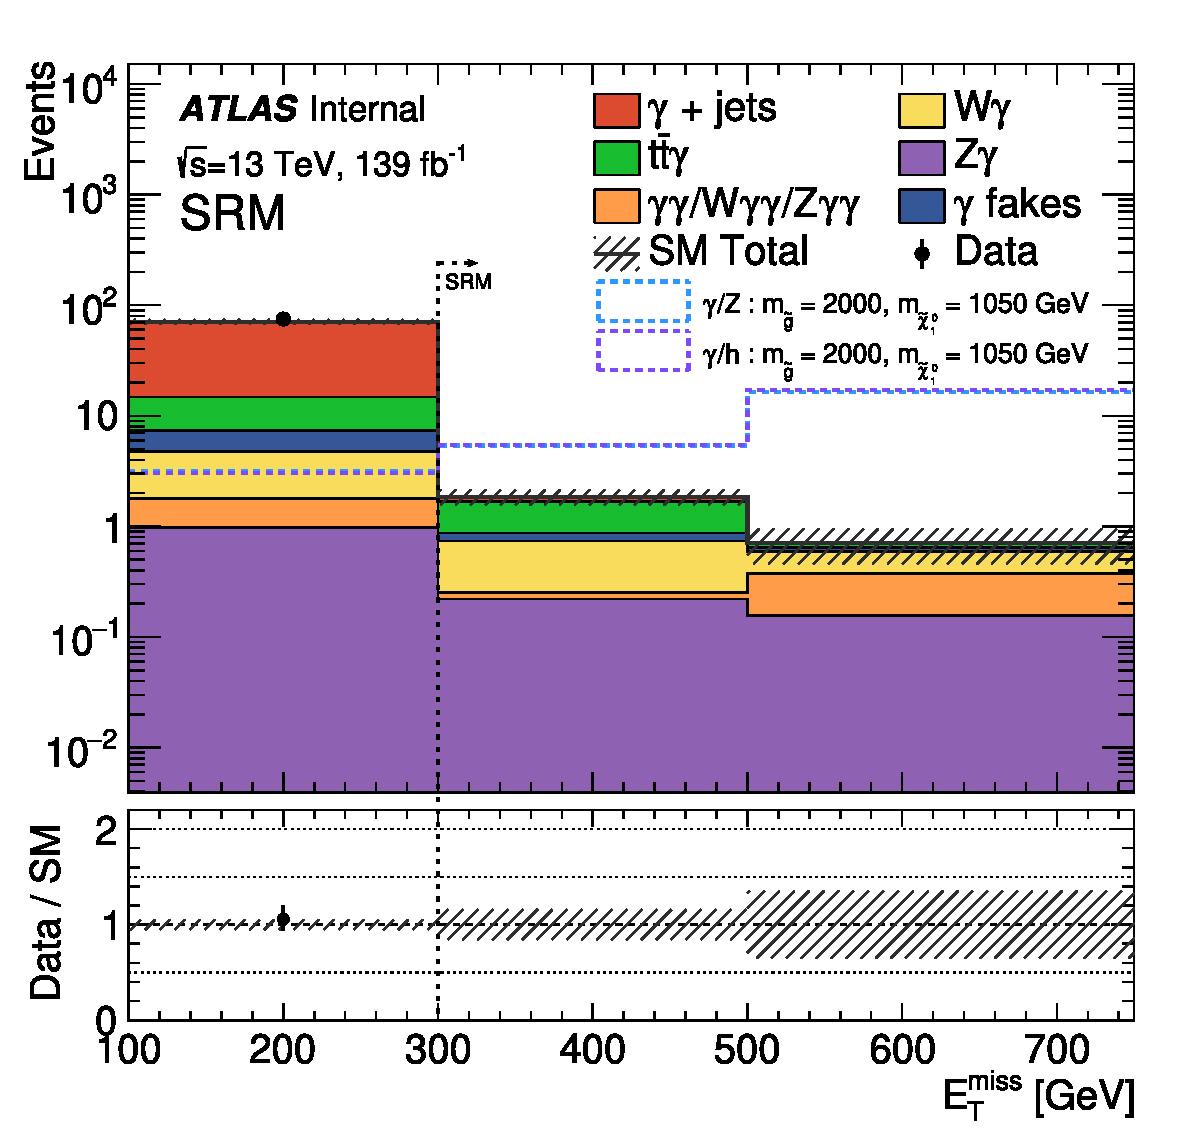
\includegraphics[width=0.5\textwidth]{images_tmp/sigReg_SRM_fr2_met_et.pdf}
   \includegraphics[width=0.5\textwidth]{images_tmp/sigReg_SRH_fr2_met_et.pdf}
   \caption{Distribución de \met\ para las regiones de señal SRL (izquierda), SRM (derecha) y SRH (abajo).}
   \label{fig:met_n-1_SRL_SRM_SRH_fr2}
 \end{center}
\end{figure}

El ajuste de solo fondo utilizado en las secciones anteriores para estimar el fondo utilizando las CR, se puede ampliar para incluir las SR y realizar pruebas de hipótesis, utilizando un enfoque de razón de probabilidad de registro de perfil (LLR), sobre la compatibilidad del número observado de eventos con el SM, para establecer límites en las secciones transversales visibles y los límites de exclusión en modelos SUSY específicos.

% \begin{table}[ht!]
%   \centering
%   \caption{Observed events and background estimates (post-fit) in the SRL, SRM and SRH signal regions. The uncertainties in the SM background are both systematic and statistical.}
%   \input{tables/fr2_unblind/table_yields_SRs.tex}
%   \label{tab:fit_result_sr}
% \end{table}

% \begin{figure}[!hb]
%    \begin{center}
%    \subfloat[SRL]{\includegraphics[width=0.5\textwidth]{figures/ATLAS_preliminary/sigReg_SRL_fr2_met_et.pdf}}%
%    \subfloat[SRM]{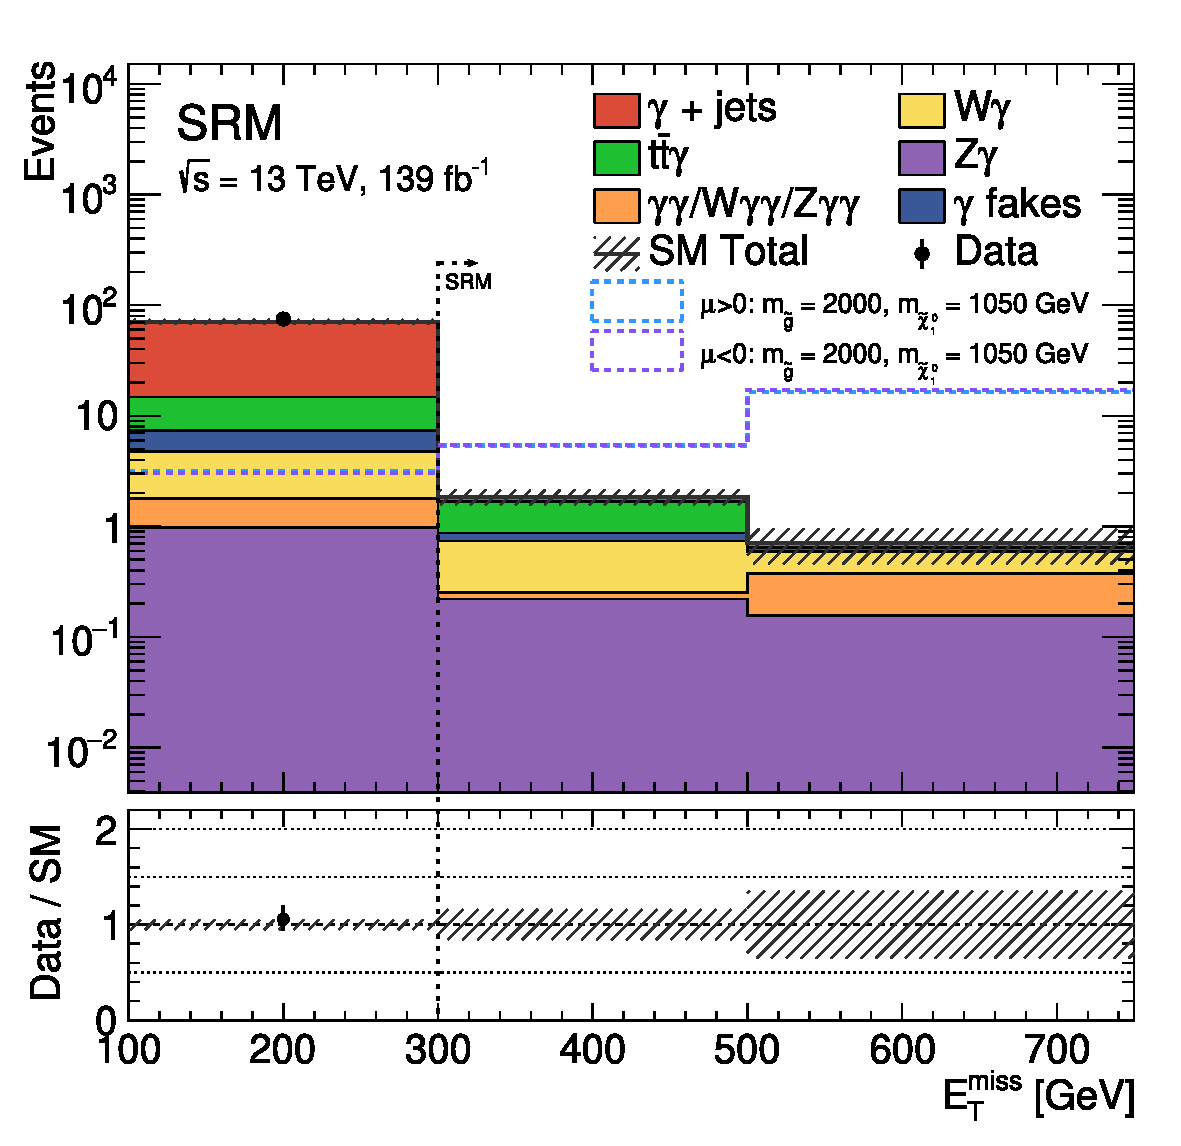
\includegraphics[width=0.5\textwidth]{figures/ATLAS_preliminary/sigReg_SRM_fr2_met_et.pdf}}\\
%    \subfloat[SRH]{\includegraphics[width=0.5\textwidth]{figures/ATLAS_preliminary/sigReg_SRH_fr2_met_et.pdf}}
%    \caption{Observed (points with error bars) and expected background (solid histograms) distributions for \MET\ in the signal region SRL (a), SRM (b) and SRH (c) after the background-only fit. The predicted signal distributions for the two models with a gluino mass of 2000~\GeV\ and neutralino mass of 250~\GeV\ (SRL), 1050~\GeV\ (SRM) or 1950~\GeV\ (SRH) are also shown for comparison. The uncertainties in the SM background are only statistical.}
%    \label{fig:met_n-1_SRL_SRM_SRH_fr2}
%  \end{center}
% \end{figure}


El ajuste se basa en las SR y CR enumerados en la Tabla
\ref{tab:sr_selection} y \ref{tab:CR_VR_selection} y tiene en cuenta todos las
incertidumbres sistemáticas discutidas en la Sección \ref{sec:uncertainties}, tratadas como parámetros de nuisanse distribuidas normalmente. Con el ajuste simultáneo en
las CR y SR se obtiene factores de normalización comunes para cada uno de los fondos de {\wph},
{\ttbarph} y QCD {\phj}. Cada incertidumbre experimental se trata como totalmente correlacionada entre las CR y el SR correspondiente, y se consideran los procesos físicos. Los sistemáticos de la teoría se tratan como correlacionados entre las diferentes regiones pero no correlacionada entre las muestras de fondo.

El número de eventos en cada SR para los datos y las contribuciones de los diferentes antecedentes del SM se muestran en la Tabla \ref{tab:fit_result_sr}. Dado que no se observa un exceso significativo por encima del fondo SM en los SR, estos se utilizan para establecer límites en el número de nuevos eventos físicos (límites independientes del modelo) y en los parámetros de los modelos de señal GGM descritos en la Sección \ref{sec:signal}.

Los límites independientes del modelo sobre el número de eventos del SM en cada SR se enumeran en la Tabla \ref{tab:model_indep_ul}, junto con el $p$-value ($p_{0}$), definido como la probabilidad de observar al menos el rendimiento del evento observado cuando asumiendo que no hay señal presente, y la correspondiente significado gaussiano Z. También
se muestra el límite superior del nivel de confianza del 95 \% en la sección transversal visible $\sigma \times A \times \epsilon$, obtenido al normalizar el límite superior al número de eventos de señal con la luminosidad integrada, donde $\sigma$ es la sección transversal de producción para una señal más allá de SM (BSM), $A$ es la aceptación (fracción de eventos con objetos que pasan todas las selecciones cinemáticas a nivel de partículas) y $\epsilon$ es la eficiencia (fracción de los eventos que se observaría después de la reconstrucción del detector).
Para SRL y SRM, $p_{0}$ tiene un límite de $0,5$ debido al hecho de que las predicciones superan los datos. Para SRH, el valor de descubrimiento $p$ es 0.09, lo que significa que estas observaciones son compatibles con la hipótesis de solo fondo. Para SRM y SRH, la diferencia en los límites esperados, que tienen el mismo número de eventos esperados y una incertidumbre similar, se ve afectada por el número de eventos observados \cite{Cowan:2010js}. Según el número de eventos observados en los SR y la expectativa de fondo, se establecen límites superiores con un nivel de confianza (CL) del 95 \% para cada SR en el número de eventos de cualquier escenario de la física de BSM.
El límite más estricto observado es para SRM, donde se excluyen las secciones transversales visibles superiores a $0,022$ fb.

Los límite de exclusión para modelos de señal SUSY específicos se basa en los estadísticos de prueba del profile likelihood, y se obtiene de un ajuste simultáneo en las contribuciones del SM y el modelo bajo estudio en una región de señal dada y sus regiones de control de fondo asociadas, que son todas por diseño estadísticamente independiente. Estos límites unilaterales se establecen en el 95 \% CL usando la receta $\mathrm{CL}_s$.
El límite de exclusión observado se calcula con la eficiencia de la señal correspondiente a la sección transversal nominal de la teoría $\pm 1 \sigma$. Los límites de exclusión combinados se muestran en la Figura \ref{fig:limit_plot_combined}, para cada modelo de señal considerado. Estos se obtienen con experimentos de pseudodatos y utilizando la región de señal con la mejor sensibilidad esperada en cada punto.
La línea continua negra corresponde a los límites esperados al 95 \% CL, con las
bandas amarillas que indican las exclusiones de 1 $\sigma$ debido a
incertidumbres de la teoría de fondo. Los límites observados están indicados por medio
curvas rojas, el contorno sólido representa el límite nominal, y las líneas punteadas se obtienen variando la sección transversal de la señal según el valor teórico.

\begin{figure}[ht!]
  \centering
  \includegraphics[width=0.5\textwidth]{images_tmp/contour_plot_gH_BestSR.pdf}
  \caption{Límites observados y esperados en el plano de masas del gluíno-neutralino a 95\% CL usando en cada punto la región de señal con mejor sensibilidad.}
  \label{fig:limit_plot_combined}
\end{figure}

Los límites en este artículo extienden entre 200 y 400 ~ \gev\ en la masa de gluino a los alcanzados en la búsqueda anterior \cite{SUSY-2016-27} para el modelo de señal $\gamma/Z$. Con respecto al modelo de señal $\gamma/h$, la búsqueda anterior \cite{SUSY-2014-01} se realizó en Run-1 con un plano de masa ligeramente diferente estableciendo un límite alrededor de 1.2 ~ \tev\ para la masa de gluino. En el presente estudio, los límites de este modelo amplían los resultados anteriores en casi 1 ~ \tev.
Para ambos modelos, los límites más estrictos de la masa de gluino se establecen en 2,4 ~ \tev\ para una masa de neutralino de 1,3/1,4 ~ \tev. Además, se alcanza un límite superior general en la masa de gluino de 2.2 ~ \tev \, para todas las masas del neutralino, con la excepción de una masa de neutralino muy baja de 150 ~ \gev\ donde el alcance en $m_{\ninoone}$ es 2050/2100 ~ \gev, como se esperaba debido a la baja aceptación de la señal del análisis en esta región.


\begin{table}[!h]
  \centering
  \caption{Resumen del número de eventos observados incluynedo los límites con 95\% de CL en la sección eficaz visible y en el número de eventos observados.}

  \begin{tabular}{lccccccc}
    \hline
    \hline
    Signal Region & $N_{\mathrm{obs}}$  & $N_{\mathrm{exp}}$  & $\langle\epsilon{\sigma}\rangle_{\mathrm{obs}}^{95}$ [fb]  & $\langle\epsilon{\sigma}\rangle_{\mathrm{exp}}^{95}$ [fb] & $S_{\mathrm{obs}}^{95}$  & $S_{\mathrm{exp}}^{95}$ & $p_{0}$(Z)\\
    \hline
    SRL  &   2   & $2.67 \pm 0.75$  &   0.034   &   $0.034^{+0.016}_{-0.009}$   &   4.73   &   $4.7^{+2.2}_{-1.2}$    &    0.50 (0.00)  \\
    SRM  &   0   & $2.55 \pm 0.64$  &   0.022   &   $0.033^{+0.013}_{-0.008}$   &   3      &   $4.6^{+1.8}_{-1.1}$    &    0.50 (0.00)  \\
    SRH  &   5   & $2.55 \pm 0.44$  &   0.054   &   $0.035^{+0.014}_{-0.010}$   &   7.55   &   $4.8^{+1.9}_{-1.4}$    &    0.09 (1.32)  \\
    \hline
    \hline
  \end{tabular}
  \label{tab:model_indep_ul}
\end{table}

% \begin{figure}[ht!]
%   \centering
%   \subfloat[$\gamma/Z$ model]{\includegraphics[width=0.5\textwidth]{figures/ATLAS_preliminary/contour_plot_gZ_BestSR.pdf}}%
%   \subfloat[$\gamma/h$ model]{\includegraphics[width=0.5\textwidth]{figures/ATLAS_preliminary/contour_plot_gH_BestSR.pdf}}

%   \caption{

%   Límites de excñusión observados y esperados en el plano de masas del lguino-neutralino

% }
%   \label{fig:limit_plot_combined}
% \end{figure}
